\question A helicopter flies to the right with a constant speed of 12 m/s, just above the surface of the Earth. A 900 kg package is suspended by a cable below the helicopter. The package is moving with the same constant velocity as the helicopter, but the force of the air against the package causes it to lag slightly behind the position of the helicopter, so that the cable makes a slight angle $\theta=22^\circ$ with respect to the vertical direction.
\begin{center}
	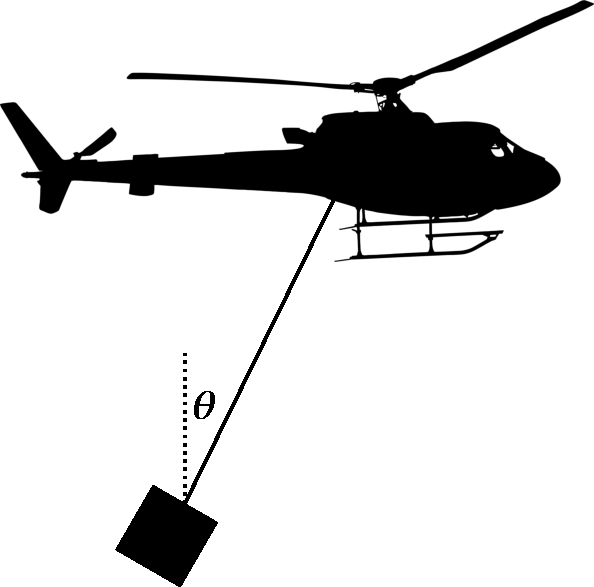
\includegraphics[width=5cm]{helicopter.pdf}
\end{center}

\begin{parts}
	\part[5] Draw a free-body diagram representing the forces acting on the package
	\vspace{4cm}
	\part[15] The strength of the cable is listed as 9300 N. Is the cable strong enough to support the package under these circumstances?
\end{parts}